% ============================================================
%  Regime-Aware Dynamic Asset Allocation --- 10-minute talk
%  Author: Tyler Pellek (tp5523@princeton.edu)
% ============================================================
\documentclass[10pt, aspectratio=169]{beamer}

% ------------------- packages -------------------
\usepackage{amsmath, amssymb, amsthm, mathtools}
\usepackage{booktabs}
\usepackage{graphicx}
\usepackage{xcolor}
\usepackage{tikz}
\usetikzlibrary{positioning, arrows.meta, shapes.geometric, fit}

% ------------------- theme ----------------------
\usetheme{metropolis}        % fallback: comment out if metropolis is not installed
% \usetheme{Boadilla}
% \usecolortheme{seahorse}

\definecolor{ParaBlue}{HTML}{0072B2}
\definecolor{ParaOrange}{HTML}{D55E00}
\definecolor{ParaGreen}{HTML}{009E73}
\definecolor{ParaGray}{HTML}{555555}

\setbeamercolor{frametitle}{bg=ParaBlue, fg=white}
\setbeamercolor{progress bar}{fg=ParaBlue}
\setbeamercolor{title separator}{fg=ParaBlue}
\setbeamercolor{alerted text}{fg=ParaOrange}

\setbeamerfont{frametitle}{size=\large, series=\bfseries}

% ------------------- macros ---------------------
\newcommand{\R}{\mathbb{R}}
\newcommand{\E}{\mathbb{E}}
\newcommand{\Sig}{\boldsymbol{\Sigma}}
\newcommand{\bmu}{\boldsymbol{\mu}}
\newcommand{\br}{\mathbf{r}}
\newcommand{\bw}{\mathbf{w}}
\newcommand{\bB}{\mathbf{B}}
\newcommand{\bF}{\mathbf{F}}
\newcommand{\bD}{\mathbf{D}}
\newcommand{\CTX}{[\mathrm{CTX}]}

\title{Regime-Aware Dynamic Asset Allocation}
\subtitle{A Cross-Asset Transformer with Factor-Structured Covariance Forecasting}
\author{Tyler Pellek}
\institute{Princeton University \\ \texttt{tp5523@princeton.edu}}
\date{\today}

\begin{document}

% ============================================================
%  Slide 1: Title
% ============================================================
\maketitle

% ============================================================
%  Slide 2: Motivation --- asymmetric correlation
% ============================================================
\begin{frame}{Motivation: Asymmetric Correlation}
\textbf{Markowitz portfolio theory} reduces asset allocation to two inputs:
\[
\bw^\star = \arg\min_{\bw}\; -\bmu^\top \bw + \tfrac{\gamma}{2}\,\bw^\top \Sig \bw
\quad\text{s.t.}\ \mathbf{1}^\top \bw = 1.
\]
The covariance $\Sig$ is what drives diversification.
\vspace{0.4em}
\begin{alertblock}{The catch}
$\Sig$ is \emph{not} stationary. Stock correlations \textbf{rise sharply during downturns} --- precisely when diversification matters most.
\end{alertblock}
\vspace{0.3em}
\textbf{Asymmetric correlation} \,(Longin \& Solnik, 2001):
\begin{itemize}
  \item Pairwise correlations among US equities: $\sim 0.3$ in calm regimes
  \item $\sim 0.8$ in crisis regimes (e.g., 2008, March 2020)
\end{itemize}
A portfolio diversified under the calm-regime $\Sig$ is \textbf{undiversified} the moment a regime shifts.
\end{frame}

% ============================================================
%  Slide 3: What classical methods miss
% ============================================================
\begin{frame}{What Classical $\Sig$ Estimators Miss}
\begin{itemize}
  \item \textbf{Sample covariance} (rolling window): backward-looking, smooth. Catches up to a regime change weeks late.
  \item \textbf{Ledoit--Wolf shrinkage}: stabilizes the estimate but offers no regime-conditional structure.
  \item \textbf{DCC-GARCH}: time-varying, but parametric and slow to adapt.
  \item \textbf{Risk-parity / inverse-vol}: dispenses with $\bmu$ and $\Sig$ jointly; uses only marginal vols.
\end{itemize}
\vspace{0.5em}
\textbf{None of these condition $\Sig$ on the current macroeconomic state.}
\vspace{0.5em}
\begin{block}{Project goal}
Build a $\Sig$ estimator that is \textbf{conditional on macro regime}, learned from data, and produces a \textbf{richer covariance signal} than any of the classical alternatives --- then verify it improves out-of-sample risk-adjusted return.
\end{block}
\end{frame}

% ============================================================
%  Slide 4: Pipeline overview
% ============================================================
\begin{frame}{Pipeline: Macro $\to$ $\Sig_t$ $\to$ Weights}
\begin{center}
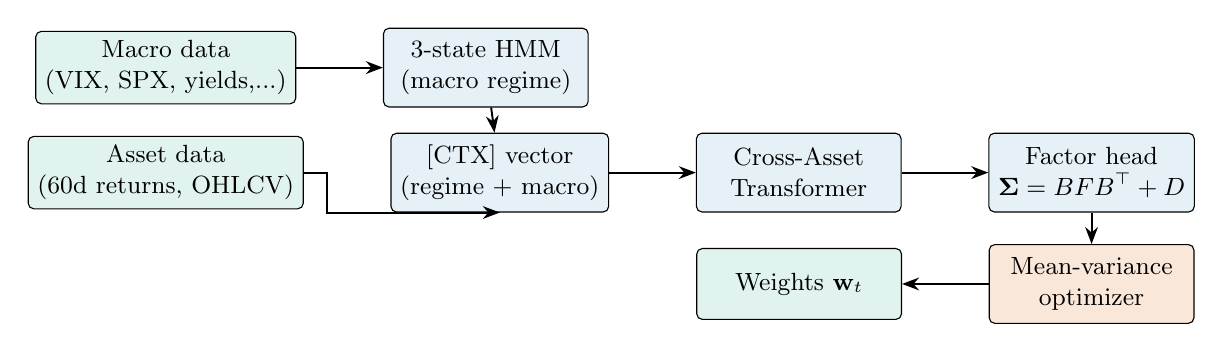
\begin{tikzpicture}[
  font=\small,
  box/.style={draw, rounded corners=2pt, align=center, minimum height=1.0cm, minimum width=2.6cm, fill=ParaBlue!10},
  data/.style={draw, rounded corners=2pt, align=center, minimum height=0.9cm, minimum width=2.6cm, fill=ParaGreen!12},
  arr/.style={-Stealth, line width=0.7pt},
  every node/.style={anchor=center}
]
\node[data] (macro) {Macro data\\(VIX, SPX, yields,...)};
\node[data, below=0.4cm of macro] (asset) {Asset data\\(60d returns, OHLCV)};
\node[box, right=1.1cm of macro] (hmm) {3-state HMM\\(macro regime)};
\node[box, right=1.1cm of asset] (ctx) {[CTX] vector\\(regime + macro)};
\node[box, right=1.1cm of ctx] (tr) {Cross-Asset\\Transformer};
\node[box, right=1.1cm of tr] (head) {Factor head\\$\Sig = BFB^\top + D$};
\node[box, below=0.4cm of head, fill=ParaOrange!15] (opt) {Mean-variance\\optimizer};
\node[data, left=1.1cm of opt] (w) {Weights $\bw_t$};
\draw[arr] (macro) -- (hmm);
\draw[arr] (hmm) -- (ctx);
\draw[arr] (asset.east) -- ++(0.3,0) |- (ctx.south);
\draw[arr] (ctx) -- (tr);
\draw[arr] (tr) -- (head);
\draw[arr] (head) -- (opt);
\draw[arr] (opt) -- (w);
\end{tikzpicture}
\end{center}
\vspace{0.2em}
\textbf{Three learned components}: HMM (fit by EM), Transformer (trained by SGD on Gaussian NLL), and an explicit convex optimizer.
\end{frame}

% ============================================================
%  Slide 5: Data and universe
% ============================================================
\begin{frame}{Data and Universe}
\textbf{Universe}: 16 US mega-cap technology equities
\begin{center}\footnotesize
AAPL, MSFT, GOOGL, AMZN, META\,(FB), NFLX, NVDA, TSLA,\\
ADBE, CRM, ORCL, INTC, CSCO, QCOM, IBM, TXN
\end{center}
\vspace{-0.3em}
\textbf{Data}
\begin{itemize}\setlength{\itemsep}{2pt}
  \item Daily OHLCV from Kaggle \texttt{jacksoncrow/stock-market-dataset} (through Apr 2020),
        extended to Dec 2024 via \texttt{yfinance}.
  \item Macro: VIX, SPX, 3m/10y/30y Treasury yields, DXY, crude oil, HYG/TLT credit proxy.
  \item Total time series: \textbf{5{,}738 trading days} (2003-01-02 $\to$ 2024-12-30).
  \item Availability mask: TSLA enters 2010-06, META 2012-05 (universe grows 14 $\to$ 16).
\end{itemize}
\vspace{0.1em}
\textbf{Backtest window}
\begin{itemize}\setlength{\itemsep}{2pt}
  \item 2008-01-02 through 2024-12-30 (17 years), \textbf{4{,}417 out-of-sample days}.
  \item \textbf{897 weekly rebalance decisions} (horizon $h=5$ trading days).
  \item \textbf{18 walk-forward folds}, each test window = 252 days $\approx$ 1 year.
\end{itemize}
\end{frame}

% ============================================================
%  Slide 6: Input vectors
% ============================================================
\begin{frame}{Model Inputs: One [CTX] Token + 16 Asset Tokens}
\begin{columns}[T,onlytextwidth]
\begin{column}{0.52\textwidth}
\textbf{Asset token (66-d, per stock):}
\begin{itemize}\setlength{\itemsep}{2pt}\footnotesize
  \item 60 trailing daily log returns
  \item rolling 60-day realized volatility
  \item previous portfolio weight $w_{t-1, i}$
  \item 4 OHLCV-derived features:
    \begin{itemize}\footnotesize
      \item intraday range $(H{-}L)/C$
      \item intraday return $(C{-}O)/O$
      \item overnight gap $(O{-}C_{\text{prev}})/C_{\text{prev}}$
      \item volume $z$-score
    \end{itemize}
\end{itemize}
\end{column}
\begin{column}{0.48\textwidth}
\textbf{[CTX] token (16-d, shared):}
\begin{itemize}\setlength{\itemsep}{2pt}\footnotesize
  \item 3 HMM regime posteriors (calm / mid / stress)
  \item VIX level + 60-day log change
  \item SPX 60-day return
  \item 10y Treasury yield + 60-day change
  \item DXY 60-day return
  \item Crude oil 60-day return
  \item HYG/TLT credit spread + change
  \item 10y$-$3m \& 30y$-$10y term spreads + changes
\end{itemize}
\end{column}
\end{columns}
\vspace{0.6em}
Each token projects through a separate linear layer into a \textbf{shared 192-d model space}; the 17 vectors then enter a 5-layer transformer.
\end{frame}

% ============================================================
%  Slide 7: HMM
% ============================================================
\begin{frame}{Hidden Markov Macro Regime Detector}
\textbf{Observation} per day: 2-d vector $X_t = (\text{SPX log return},\; \log \text{VIX})$
\vspace{0.3em}\\
\textbf{Model:} 3-state Gaussian HMM, full covariance per state.
\[
P(X_t \mid s_t = k) = \mathcal{N}(X_t \mid \mu_k, \Sigma_k),
\quad
P(s_t \mid s_{t-1}) = A_{s_{t-1}, s_t}.
\]
\textbf{Fit} by Baum-Welch (EM); \textbf{outside the gradient graph} of the transformer.
\vspace{0.2em}
\begin{itemize}\setlength{\itemsep}{1pt}\footnotesize
  \item State 0 = lowest mean log-VIX (\textbf{calm})
  \item State 1 = middle (\textbf{mid})
  \item State 2 = highest (\textbf{stress})
  \item Post-fit relabeling by mean log-VIX gives stable semantics across re-fits.
\end{itemize}
\vspace{0.2em}
\textbf{Output}: 3-vector $[\,P(\text{calm}_t),\,P(\text{mid}_t),\,P(\text{stress}_t)\,]$, fed into the [CTX] token.
\end{frame}

% ============================================================
%  Slide 8: Transformer
% ============================================================
\begin{frame}{Cross-Asset Transformer}
\textbf{Sequence layout}: 1 [CTX] + 16 asset tokens $\Rightarrow$ length-17 sequence in 192-d.
\vspace{0.2em}
\begin{itemize}\setlength{\itemsep}{2pt}
  \item \textbf{Two projections}: $W_{\CTX}\!\in\!\R^{192\times 16}$ for the context, $W_{\text{asset}}\!\in\!\R^{192\times 66}$ \textbf{shared across all 16 assets}.
  \item Asset identity carried by \textbf{learned positional embeddings} $p_1,\dots,p_{16}$.
  \item 5 pre-LN transformer blocks; 8 heads; FF expansion $\times 4$; dropout 0.15.
  \item Self-attention lets every asset attend to every other asset \textbf{and} to the [CTX] row $\Rightarrow$ cross-asset interactions are dynamic, input-dependent.
  \item \textbf{Mask}: inactive assets (e.g., TSLA pre-2010) excluded at every attention layer.
\end{itemize}
\vspace{0.3em}
\textbf{Total parameters} $\approx 1.8 \times 10^{6}$, all trained jointly under one loss.
\end{frame}

% ============================================================
%  Slide 9: Factor head
% ============================================================
\begin{frame}{Factor-Structured Covariance Head}
A full Cholesky parametrization would predict $N(N{+}1)/2 = 136$ entries per snapshot ---
too many for $\sim$500--2{,}500 training points per fold.

\vspace{0.3em}
\textbf{Rank-4 factor structure}:
\[
\boxed{\;\Sig_t \;=\; \bB_t\, \bF_t\, \bB_t^\top \;+\; \bD_t\;}
\]
\begin{itemize}\setlength{\itemsep}{2pt}\footnotesize
  \item $\bB_t \in \R^{16\times 4}$ (factor loadings): linear head on each asset row.
  \item $\bD_t = \mathrm{diag}(d_{t,i}^2)$: scalar head + softplus $\to$ positive idiosyncratic variance.
  \item $\bF_t \in \R^{4\times 4}$: linear head on the \textbf{[CTX] row}, parameterized as $\bF_t^{1/2}(\bF_t^{1/2})^\top$.
\end{itemize}
\vspace{0.2em}
\textbf{Why this matters}: $\bF_t$ is the only component derived from the macro/[CTX] state. The factor structure is therefore \textbf{explicitly regime-conditioned} --- this is where asymmetric correlation enters the model.
\end{frame}

% ============================================================
%  Slide 10: Objective function
% ============================================================
\begin{frame}{Training Objective: Gaussian NLL}
For each snapshot, predict $(\bmu_t, \Sig_t)$ and score against the realized 5-day forward return $\br_{t, t+h}$:
\vspace{-0.2em}
\[
\mathcal{L}_t = \frac{1}{2|\mathcal{A}_t|}\left[\,|\mathcal{A}_t|\log(2\pi) + \log\det \Sig_t + (\br_{t,t+h} - \bmu_t)^\top \Sig_t^{-1} (\br_{t,t+h} - \bmu_t)\,\right]
\]
\vspace{-0.3em}
\textbf{Why this loss?}
\begin{itemize}\setlength{\itemsep}{2pt}\footnotesize
  \item \textbf{Principled}: maximum likelihood under a multivariate Gaussian.
  \item \textbf{Couples $\bmu$ and $\Sig$}: both heads train under one loss; the quadratic form $r^\top\Sig^{-1}r$ shrinks residuals, the $\log\det\Sig$ term prevents the model from inflating $\Sig$ arbitrarily.
  \item \textbf{Per-active-asset normalization} stabilizes loss magnitude as the universe grows (14 $\to$ 16).
  \item \textbf{Cholesky parameterization} of $\Sig$ makes $\log\det$ and $\Sig^{-1}$ computable in $O(N^2)$ via triangular solves.
\end{itemize}
\textbf{Optimizer}: AdamW, $\eta=3\!\times\!10^{-4}$, weight decay $5\!\times\!10^{-4}$, gradient clip 1.0, cosine annealing, 6-epoch early-stopping patience.
\end{frame}

% ============================================================
%  Slide 11: Walk-forward + warm-start
% ============================================================
\begin{frame}{Walk-Forward Training + Warm-Start Fine-Tuning}
\textbf{18 expanding-window folds}; fold $f$ trains on $[t_{\text{start}},\,t_f]$, tests on the next 252 days.
\vspace{0.2em}
\begin{center}
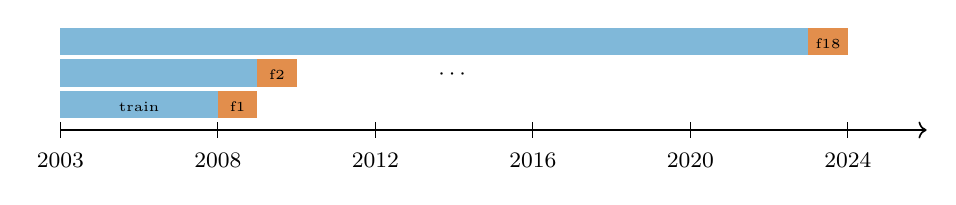
\begin{tikzpicture}[font=\footnotesize]
  \draw[->, line width=0.6pt] (0,0) -- (11,0);
  \foreach \x/\lbl in {0/2003, 2/2008, 4/2012, 6/2016, 8/2020, 10/2024}
    \draw (\x,0.1) -- (\x,-0.1) node[below=2pt] {\lbl};
  \fill[ParaBlue!50] (0,0.15) rectangle (2,0.5); \node at (1,0.3) {\tiny train};
  \fill[ParaOrange!70] (2,0.15) rectangle (2.5,0.5); \node at (2.25,0.3) {\tiny f1};
  \fill[ParaBlue!50] (0,0.55) rectangle (2.5,0.9);
  \fill[ParaOrange!70] (2.5,0.55) rectangle (3,0.9); \node at (2.75,0.7) {\tiny f2};
  \node at (5,0.7) {$\cdots$};
  \fill[ParaBlue!50] (0,0.95) rectangle (9.5,1.3);
  \fill[ParaOrange!70] (9.5,0.95) rectangle (10,1.3); \node at (9.75,1.1) {\tiny f18};
\end{tikzpicture}
\end{center}
\vspace{0.1em}
\textbf{Per-fold internal split}: last 15\% of train period serves as \textbf{validation}; best-validation weights restored at fold end.
\vspace{0.3em}
\textbf{Warm-start}:
\begin{itemize}\setlength{\itemsep}{2pt}\footnotesize
  \item Fold 0: random init, $\sim$30 epochs.
  \item Fold $f \geq 1$: initialize from fold $(f{-}1)$ weights, LR scaled by $\eta_{\text{warm}}=0.5$.
  \item HMM is \textbf{re-fit per fold} (not warm-started) using only data up to the fold's training cutoff.
  \item Ablation: cold-init each fold collapses Sharpe from 1.02 $\to$ 0.27.
\end{itemize}
\end{frame}

% ============================================================
%  Slide 12: Inference pipeline
% ============================================================
\begin{frame}{Inference Pipeline}
At each weekly rebalance date $t$:
\vspace{0.3em}
\begin{enumerate}\setlength{\itemsep}{3pt}
  \item Update HMM posteriors $\to$ [CTX] vector.
  \item Forward pass through transformer $\to (\bmu_t^{\text{model}}, \Sig_t^{\text{model}})$.
  \item \textbf{Shrinkage} (Ledoit-Wolf-style):
    \[
    \Sig_t^{\text{final}} = \alpha\,\Sig_t^{\text{model}} + (1-\alpha)\,\Sig_t^{\text{sample}},
    \quad \alpha = 0.7
    \]
  \item Replace learned $\bmu$ with a \textbf{60-day sample mean} (justified by ablation).
  \item Solve the convex program with Clarabel via CVXPY:
\end{enumerate}
\vspace{-0.4em}
\[
\bw_t^\star = \arg\min_{\bw}\; -\bmu_t^\top\bw + \tfrac{\gamma}{2}\bw^\top\!\Sig_t^{\text{final}}\bw + \lambda_{\text{TO}}\|\bw - \bw_{t-1}\|_1
\]
\vspace{-1.2em}
\[
\text{s.t.}\quad \mathbf{1}^\top\bw = 1,\quad 0 \le w_i \le 0.20,\quad \sqrt{\bw^\top \Sig_t^{\text{final}} \bw} \le 0.040.
\]
The weekly volatility cap is the explicit risk-control lever that converts ``good $\Sig$ forecast'' into ``small drawdown.''
\end{frame}

% ============================================================
%  Slide 13: Results --- equity
% ============================================================
\begin{frame}{Results: Out-of-Sample Equity Curves}
\begin{center}
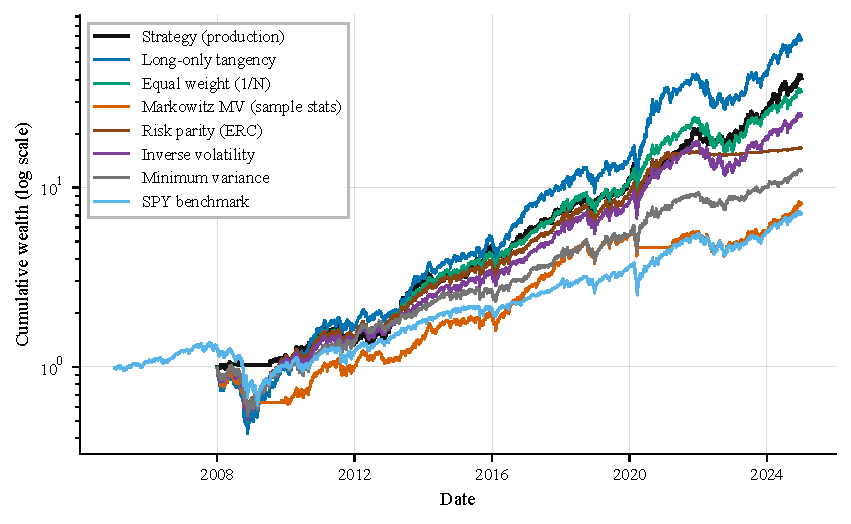
\includegraphics[width=0.92\linewidth]{fig_equity.pdf}
\end{center}
\vspace{-0.3em}
\footnotesize
The long-only tangency baseline finishes at higher cumulative wealth, but with $-57.6\%$ drawdown vs.\ our $-25.1\%$. \textbf{Our strategy is the risk-adjusted leader, not the absolute-return leader.}
\end{frame}

% ============================================================
%  Slide 14: Results --- drawdown
% ============================================================
\begin{frame}{Results: Drawdown vs.\ Long-Only Tangency Baseline}
\begin{center}
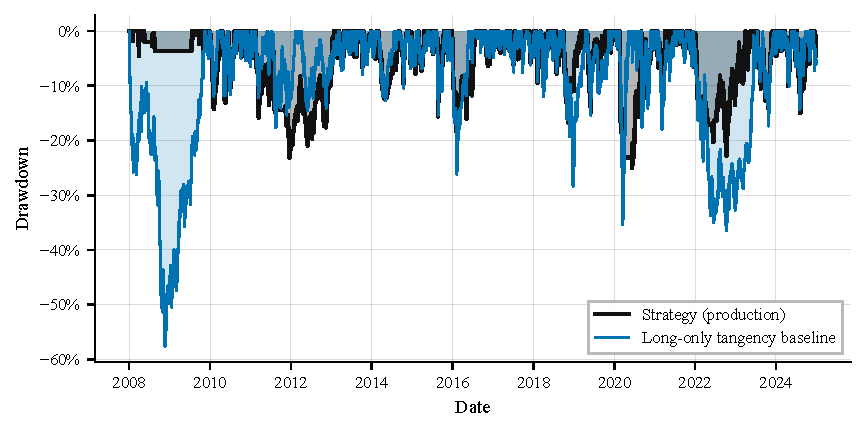
\includegraphics[width=0.92\linewidth]{fig_drawdown_tangency.pdf}
\end{center}
\vspace{-0.3em}
\footnotesize
The tangency baseline finishes at higher cumulative wealth, but at $-57.6\%$ maximum drawdown (2008-11-20). Our strategy's MaxDD is $-25.1\%$ (2020-06-11), and only $-4.5\%$ across the 2008 GFC --- the regime-conditional $\Sig$ tells the optimizer to step out when correlations spike.
\end{frame}

% ============================================================
%  Slide 15: Results --- metrics table
% ============================================================
\begin{frame}{Results: Risk-Adjusted Performance Ranking}
\centering\small
\begin{tabular}{lrrrr}
\toprule
Strategy & CAGR & Sharpe & MaxDD & Calmar \\
\midrule
\textbf{Production (ours)}  & \textbf{23.6\%} & \textbf{1.21} & \textbf{$-$25.1\%} & \textbf{0.94} \\
Long-only tangency          & 27.0\%          & 1.02          & $-$57.6\%          & 0.47          \\
Equal-weight (1/$N$)        & 22.3\%          & 0.96          & $-$51.4\%          & 0.43          \\
Inverse-volatility          & 20.1\%          & 0.91          & $-$50.1\%          & 0.40          \\
Risk-parity (ERC)           & 17.3\%          & 0.87          & $-$49.9\%          & 0.35          \\
Minimum-variance            & 15.4\%          & 0.83          & $-$47.5\%          & 0.32          \\
Sample-stats MV             & 12.6\%          & 0.71          & $-$38.9\%          & 0.32          \\
SPY benchmark               & 10.3\%          & 0.61          & $-$55.2\%          & 0.19          \\
\bottomrule
\end{tabular}
\vspace{0.6em}\\
\footnotesize
\textbf{Best Sharpe, best Calmar, smallest drawdown among all 7 baselines + SPY.}\\
Beta vs.\ SPY: 0.51; alpha (annualized): 17.6\%.
\end{frame}

% ============================================================
%  Slide 16: Negative results
% ============================================================
\begin{frame}{Negative Results: 18 Attempts, 18 Regressions}
We tried 18 architecture/optimizer modifications. \textbf{All reduced out-of-sample Sharpe.}
\vspace{0.3em}
\centering\footnotesize
\begin{tabular}{lr}
\toprule
Variant & $\Delta$ Sharpe vs.\ 1.21 \\
\midrule
12-1 Jegadeesh-Titman momentum $\bmu$            & $-0.41$ \\
Scenario-based CVaR optimizer                     & $-0.36$ \\
Long/short relaxation ($w_i \in [-0.1, 0.2]$)     & $-0.29$ \\
5-seed ensemble                                   & $-0.18$ \\
Realized-covariance auxiliary loss                & $-0.14$ \\
Cold-init each fold (no warm-start)               & $-0.94$ \\
Larger transformer ($d_{\text{model}}=320$)       & $-0.15$ \\
Daily training stride (v17b)                      & $-0.22$ \\
GNN over asset interactions                       & $-0.31$ \\
\multicolumn{2}{c}{\emph{$\cdots$ and nine more, all negative}} \\
\bottomrule
\end{tabular}
\vspace{0.5em}\\
\textbf{Interpretation}: the v7b config is a tight, opinionated local optimum. Its success comes from \textbf{constrained, low-DOF architecture}, not from flexibility.
\end{frame}

% ============================================================
%  Slide 17: Conclusion
% ============================================================
\begin{frame}{Conclusion}
\textbf{What we built}
\begin{itemize}\setlength{\itemsep}{2pt}
  \item Macro-regime-conditional covariance forecaster: HMM $+$ cross-asset Transformer $+$ factor head.
  \item Trained under Gaussian NLL on 5-day forward returns; rigorous 18-fold walk-forward protocol.
\end{itemize}
\textbf{What we found}
\begin{itemize}\setlength{\itemsep}{2pt}
  \item \textbf{Sharpe 1.21, Calmar 0.94, MaxDD $-25.1\%$} OOS over 2008--2024.
  \item Beats 7 classical baselines + SPY on every risk-adjusted metric.
  \item Architecture is brittle to perturbation --- 18 of 18 ablations regressed.
\end{itemize}
\textbf{Limitations}
\begin{itemize}\setlength{\itemsep}{2pt}\footnotesize
  \item Universe selected from a 2020 snapshot $\to$ survivorship bias.
  \item No transaction-cost model; gross-of-cost Sharpe.
  \item Single asset class (equities). Multi-asset extension untested.
\end{itemize}
\vspace{0.4em}
\begin{center}
\textbf{Thank you. Questions?}\\
\footnotesize \texttt{tp5523@princeton.edu}
\end{center}
\end{frame}

\end{document}
